
\chapter{Exact Inference in Probabilistic Graphical Models}

In the context of inference, out task is, given a joint distribution $p(X) = p(x_1, \dots, x_n)$ to compute marginals or conditionals of the distribution.

We formalize this by considering two disjoint subsets of r.v.: $y \subseteq x, z \subseteq x$ s.t. $y \cap z = \emptyset$ and $y \cup z \subseteq x$.

Given that we observe $y$, we want to compute the conditional
$$
    \begin{array}{rl}
        p(z|y = \bar{y})
        & = \sum_{x}^{}p(z,x'|y = \bar{y}) discrete r.v. \\
        & = p(z|y = \bar{y} = \int_{x}^{}p(z,x'|y = \bar{y})) continuous r.v.
    \end{array}    
$$

being $x'$ s.t. $x' \cup y \cup z = x$.

\textbf{Remark:} this summation can be of the order of $O(\mathcal{K}^m)(|x'|=m)$, hence obtaining this marginalization is computationally challenging!

Our goal is to carry out this computation efficiently, by leverage the factorization implied by the PGM.

As an example, consider a Markov Random Field where variables are connected in a chain (colored rectangles represent the cliques):
\begin{figure}[H]
    \centering
    \includegraphics[width=0.7\textwidth]{assets/fig18.png}
\end{figure}

The factorization implied by this PGM is:
$$
    p(x) = \frac{1}{Z} \cdot \psi_{1,2}(x_1, x_2)\cdot \psi_{2,3}(x_2, x_3)\dots \psi_{x_{n-1}, x_{n}}(x_{n-1}, x_n)
$$

Consider now the equivalent model in case of a Bayesian Network:

\begin{center}
    \begin{tikzpicture}
        % Nodes
        \node (x1) [circle,draw] {\(\mathbf{x_1}\)};
        \node (x2) [circle,draw, right=of x1] {\(\mathbf{x_2}\)};
        \node (x3) [circle,draw, right=of x2] {\(\mathbf{x_3}\)};
        \node (xn) [circle,draw, right=of x3] {\(\mathbf{x_n}\)};
        
        % Arrows
        \draw[->] (x1) -- (x2);
        \draw[->] (x2) -- (x3);
        \draw[dotted] (x3) -- (xn);
    \end{tikzpicture}
\end{center}

The factorization in this case reads as 
$$
    p(x) = p(x_1)\cdot p(x_2|x_1)\cdot p(x_3|x_2) \dots p(x_n|x_{n-1})
$$

\begin{observationblock}[Markov processes]
    Chain structures like the previous are common because they repre-
    sent temporal series (more specifically, they are Markov processes).
\end{observationblock}

Suppose that, given the model above, we want to compute the marginal
$$
    p(x_k) = \sum_{x_1,\dots, x_{k-1},x_{k+1},x_n}^{}p(x_1,\dots, x_n)
$$

with $1<k<n$. In principle this has complexity $O(\mathcal{K}^{n-1})$.

However, plugging the factorization implied by the Markov Random Field, we get(using the distributive laws of sum and product):
$$
\begin{array}{rl}
    p(x_k)
    & = \sum_{x_-k}^{}\frac{1}{Z}\psi_{1,2}(x_1, x_2)\dots \psi_{n-1, n}(x_{n-1}, x_n)\\
    & = \frac{1}{Z} \sum_{x_{k-1}}\psi_{k-1, k}(x_{k-1}, x_k) \dots \left[ \sum_{x_2}^{}\psi_{2,3}(x_2, x_3)\left[\sum_{x_1}^{}\psi(x_1, x_2)\right]\right] + \\
    & + \sum_{x_{k+1}}^{}\psi_{k, k+1}(x_k, x_{k+1}) \dots \left[\sum_{x_{n-1}}^{}\psi_{n-2, n-1}(x_{n-2}, x_{n-1})\left[\sum_{x_n}^{}\psi_{n-1, n}(x_{n-1, x_n})\right]\right]
\end{array}
$$

Note that complexity is now $O(n\cdot k)$, i.e. linear in $n$. 

We can define a dynamic programming algorithm, called \textbf{message-passing algorithm}, in which the information from the graph is summarized by local edge information. 

We break the chain in two parts, the past and the future w.r.t. $x_k$, and we define the following:
\begin{itemize}
    \item forward message: $\mu_\alpha(x_k) = \sum_{x_{k-1}}^{}\psi_{k-1, k}(x_{k-1}, x_k)\cdot \mu_{\alpha}(x_{k-1})$, with base case $\mu_{\alpha}(x_1) = 1$
    \item backward message: $\mu_{\beta}(x_k) = \sum_{x_{k+1}}\psi_{k, k-1}(x_k, x_{k+1})\cdot \mu_{\beta}(x_{k+1})$, with base case $\mu_{\beta}(x_n) = 1$
\end{itemize}

In this algorithm, each node sends a message to its neighbors, and the messages are computed by the above formulas.

\begin{figure}[H]
    \centering
    \includegraphics[width=0.9\textwidth]{assets/fig19.png}
    \caption{Message-passing algorithm}
\end{figure}

Once we have both $\mu_{\alpha}(x_k)$ and $\mu_{\beta}(x_k)$, we can observe that:
$$
    p(x_k) = \frac{1}{Z_k}\cdot \mu_{\alpha}(x_k)\mu_{\beta}(x_k) \propto \mu_{\alpha}(x_k)\mu_{\beta}(x_k)
$$
with the normalization constant $Z_k$ computed as $Z_k = \sum_{x_k}^{}\mu_{\alpha}(x_k)\mu_{\beta}(x_k)$.

Summarizing, the idea behind this algorithm is to start from the extremes of the chain and pass messages (forward and backward) until the other end is reached. Once there, messages are combined to obtain an (un)normalized marginal distribution.

\section{Factor Graphs}

Our goal in what follows is to extend what we have done for chains to more general graph structures, i.e. trees and politrees. In order to do so, we need to introduce the formalism of \textbf{Factor Graphs}.

The idea behind them is to expose in a more clear way what are the factors and what are the variables. For this reason, Factor Graphs are bipartite graphs (i.e. nodes are divided in two classes), in which we have:
\begin{table}[H]
    \centering
    \begin{tabular}{c|c}
        \textbf{Variable nodes} & \textbf{Factor nodes} \\
        \hline
        $x$ & $f$ \\

    \end{tabular}
\end{table}

The canonical way of represent bipartite graphs is the following:

\begin{center}
    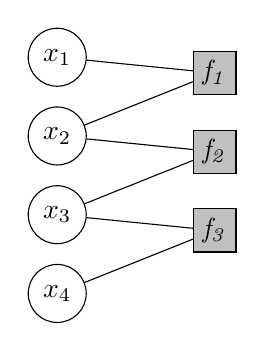
\begin{tikzpicture}
        % Nodes on the left (x variables)
        \node (x1) [circle, draw] at (0,3) {\(x_1\)};
        \node (x2) [circle, draw] at (0,2) {\(x_2\)};
        \node (x3) [circle, draw] at (0,1) {\(x_3\)};
        \node (x4) [circle, draw] at (0,0) {\(x_4\)};
        
        % Nodes on the right (f variables)
        \node (f1) [rectangle, draw, fill=gray!50] at (2,2.8) {\(\mathit{f_1}\)};
        \node (f2) [rectangle, draw, fill=gray!50] at (2,1.8) {\(\mathit{f_2}\)};
        \node (f3) [rectangle, draw, fill=gray!50] at (2,0.8) {\(\mathit{f_3}\)};
        
        % Edges
        \draw (x1) -- (f1);
        \draw (x2) -- (f1);
        \draw (x2) -- (f2);
        \draw (x3) -- (f2);
        \draw (x3) -- (f3);
        \draw (x4) -- (f3);
        
    \end{tikzpicture}
\end{center}

That is, all variable nodes are put on the left and all factor nodes on the right. 

A more convenient, equivalent, representation could be:

\begin{center}
    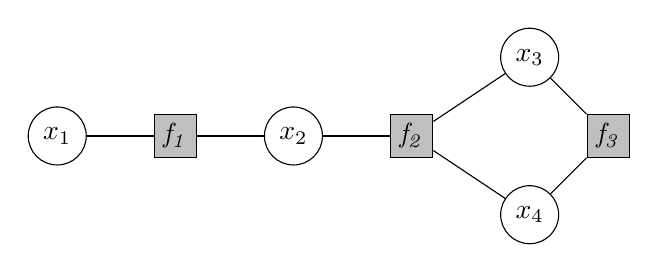
\begin{tikzpicture}
        % Nodes
        \node (x1) [circle, draw] at (0,0) {\(x_1\)};
        \node (f1) [rectangle, draw, fill=gray!50] at (1.5,0) {\(\mathit{f_1}\)};
        \node (x2) [circle, draw] at (3,0) {\(x_2\)};
        \node (f2) [rectangle, draw, fill=gray!50] at (4.5,0) {\(\mathit{f_2}\)};
        \node (x3) [circle, draw] at (6,1) {\(x_3\)};
        \node (x4) [circle, draw] at (6,-1) {\(x_4\)};
        \node (f3) [rectangle, draw, fill=gray!50] at (7,0) {\(\mathit{f_3}\)};
        
        % Edges
        \draw (x1) -- (f1);
        \draw (f1) -- (x2);
        \draw (x2) -- (f2);
        \draw (f2) -- (x3);
        \draw (f2) -- (x4);
        \draw (x3) -- (f3);
        \draw (x4) -- (f3);
    
    \end{tikzpicture}
\end{center}

\subsection{From Bayesian Networks to Factor Graphs}
Consider the following Bayesian Network:

\begin{center}
    \begin{tikzpicture}
        % Nodes
        \node (x1) [circle, draw] at (0,0) {\(x_1\)};
        \node (x2) [circle, draw] at (3,0) {\(x_2\)};
        \node (x3) [circle, draw] at (1.5,-3) {\(x_3\)};
        \node (x4) [circle, draw] at (4.5,-3) {\(x_4\)};
        \node (x5) [circle, draw] at (3,-6) {\(x_5\)};
        
        % Directed Edges
        \draw[->] (x1) -- (x3);
        \draw[->] (x2) -- (x3);
        \draw[->] (x3) -- (x5);
        \draw[->] (x4) -- (x5);
    \end{tikzpicture}
\end{center}

Which corresponds to the factorization:
$$
    \begin{array}{rl}
        p(x)
        & = p(x_1)p(x_2)p(x_3|x_1, x_2)p(x_4)p(x_5|x_3, x_4)\\
        & = f_1(x_1)f_2(x_2)f_3(x_1, x_2, x_3)f_4(x_4)f_5(x_3, x_4, x_5)
    \end{array}
$$

Fundamentally, the idea is to have a factor node (connected to the proper variable nodes) for each term of the factorization implied by the Bayesian Network.

Formally: $\forall p(x_j|pa_j) \to f_j \curvearrowright {x_j} \cup pa_j$.

Hence the Factor Graph equivalent to the Bayesian Network above is:

\begin{center}
    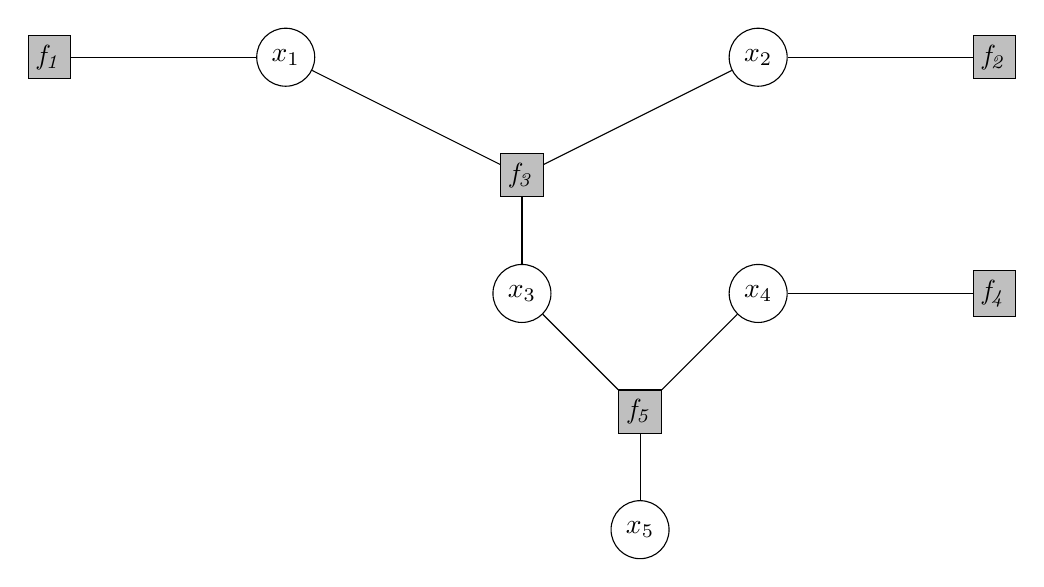
\begin{tikzpicture}
        % Nodes
        \node (x1) [circle, draw] at (0,0) {\(x_1\)};
        \node (f1) [rectangle, draw, fill=gray!50] at (-3,0) {\(\mathit{f_1}\)};
        \node (x2) [circle, draw] at (6,0) {\(x_2\)};
        \node (f2) [rectangle, draw, fill=gray!50] at (9, 0) {\(\mathit{f_2}\)};
        \node (x3) [circle, draw] at (3, -3) {\(x_3\)};
        \node (f3) [rectangle, draw, fill=gray!50] at (3, -1.5) {\(\mathit{f_3}\)};
        \node (x4) [circle, draw] at (6, -3) {\(x_4\)};
        \node (f4) [rectangle, draw, fill=gray!50] at (9, -3) {\(\mathit{f_4}\)};
        \node (x5) [circle, draw] at (4.5, -6) {\(x_5\)};
        \node (f5) [rectangle, draw, fill=gray!50] at (4.5, -4.5) {\(\mathit{f_5}\)};
        
        % Edges
        \draw (x1) -- (f1);
        \draw (x1) -- (f3);
        \draw (x2) -- (f3);
        \draw (x2) -- (f2);
        \draw (x3) -- (f3);
        \draw (x3) -- (f5);
        \draw (x4) -- (f4);
        \draw (x4) -- (f5);
        \draw (x5) -- (f5);
    
    \end{tikzpicture}
\end{center}

\subsection{From Markov Random Fields to Factor Graphs}
Consider the following Markov Random Field (rectangles correspond to the cliques):
\begin{figure}[H]
    \centering
    \includegraphics[width=0.5\textwidth]{assets/fig20.png}
\end{figure}

Which implies the factorization:
$$
    p(x) = \frac{1}{Z}\psi_1(x_1, x_2, x_3)\psi_2(x_3, x_4) = \frac{1}{Z}f_1(x_1, x_2, x_3)f_2(x_3, x_4)
$$

This leads to the following Factor Graph:
\begin{center}
    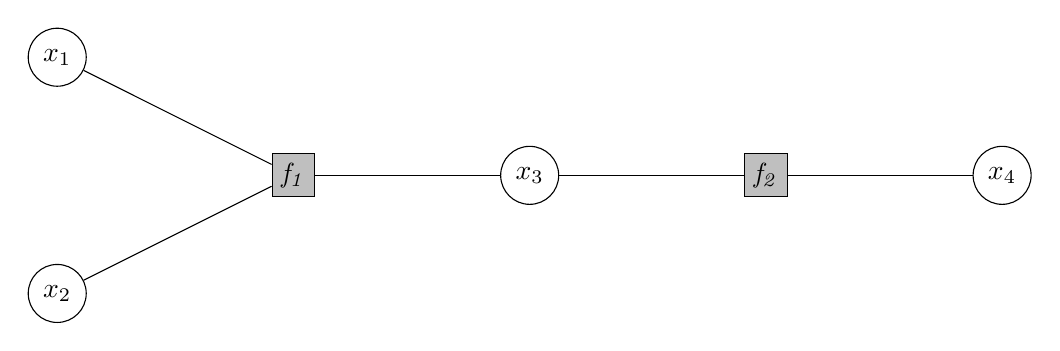
\begin{tikzpicture}
        % Nodes
        \node (x1) [circle, draw] at (-3, 1.5) {\(x_1\)};
        \node (f1) [rectangle, draw, fill=gray!50] at (0,0) {\(\mathit{f_1}\)};
        \node (x2) [circle, draw] at (-3, -1.5) {\(x_2\)};
        \node (f2) [rectangle, draw, fill=gray!50] at (6,0) {\(\mathit{f_2}\)};
        \node (x3) [circle, draw] at (3, 0) {\(x_3\)};
        \node (x4) [circle, draw] at (9, 0) {\(x_4\)};
        
        % Edges
        \draw (x1) -- (f1);
        \draw (f1) -- (x2);
        \draw (f1) -- (x3);
        \draw (f2) -- (x4);
        \draw (x3) -- (f2);
    
    \end{tikzpicture}
\end{center}

Hence, the conversion from Markov Random Fields to Factor Graphs works as: $\forall c \in \mathcal{C} \rightarrow f_c(x_c) \sim \psi_c(x_c) $ (equality does not hold because of
the normalization constant).

So, whether we are starting from a Bayesian Network or from a Markov
Random Field, we can convert our PGM into a Factor Graph and perform
message passing on it, without loss of generality.

\section{Sum Product Algotithm}

Our goal is now to do inference in Factor Graphs, generalizing to more
general graph structures what we did with chains previously. Consider
the following Factor Graph:


\begin{center}
    \begin{tikzpicture}
        % Nodes
        \node(x1) [circle, draw] at (-6, 1.5) {\(x_1\)};
        \node (f1) [rectangle, draw, fill=gray!50] at (-3,1.5) {\(\mathit{f_1}\)};
        \node (x2) [circle, draw] at (-6, -1.5) {\(x_2\)};
        \node (f2) [rectangle, draw, fill=gray!50] at (-3,-1.5) {\(\mathit{f_2}\)};
        \node (x3) [circle, draw] at (0, 0) {\(x_3\)};
        \node (f3) [rectangle, draw, fill=gray!50] at (3, -1.5) {\(\mathit{f_3}\)};
        \node (x4) [circle, draw] at (0, -3) {\(x_4\)};
        \node (x5) [circle, draw] at (6, -1.5) {\(x_5\)};
    
        % Edges
        \draw (x1) -- (f1);
        \draw (f1) -- (x3);
        
        \draw (x2) -- (f2);
        \draw (f2) -- (x3);
        
        \draw (x3) -- (f3);
        \draw (x4) -- (f3);
        
        \draw (f3) -- (x5);
    
        % Labels
        \node[left=of x1, blue] {leaf};
        \node[left=of x2, blue] {leaf};
        \node[left=of x4, blue] {leaf};
        \node[right=of x5, red] {root};
    
    \end{tikzpicture}
    \end{center}

The joint probabbility distribution implied by thie Factor Graph is:

$$
p(x) = f_1(x_1, x_3)f_2(x_2, x_3)f_3(x_3, x_4, x_5)
$$

Since the above graph is actually a tree, we can identify the \textbf{root} node  (choice is arbitrary, here it is $x_5$) and consequently the \textbf{leaves} (in the example, $x_1,x_2,x_4$). Recall that there is a unique path from the root to any of the leaves and that following all those paths we visit all the nodes in the tree.

The message passing algorithm that we are going to detail is called \textbf{Belief Propagation} and works in Factor Graphs which are trees (i.e., without any loop).

Assume that the root is the node of which we want to compute the marginal (this is not necessarily the case, indeed after performing forward and backward pass we have sufficient information to compute the marginal w.r.t. each node in graph).

So, let's consider the marginal probability w.r.t. $x_5$:

$$
\begin{array}{rl}
    p(x_5) &= \sum_{x_1,x_2,x_3,x_4} p(x_1,x_2,x_3,x_4,x_5) \\
    &= \sum_{x_3,x_4} f_3(x_3,x_4,x_5) \left[\sum_{x_1} f_1(x_1,x_3)\right]\left[\sum_{x_2} f_2(x_2,x_3)\right]
\end{array}
$$

Take $\sum_{x_1} f_1(x_1,x_3)$: we can see this as a message going from factor $f_1$ to variable $x_3$. We denote it by $\mu_{f_1 \to x_3}(x_3)$.

Analogously, $\sum_{x_2} f_2(x_2,x_3) \doteq \sum_{x_1} f_1(x_1,x_3) \cdot \sum_{x_2} f_2(x_2,x_3)$.

Finally, the full summation can be seen as a message going from factor $f_3$ to variable $x_5$, i.e. $\mu_{f_3 \to x_5}(x_5) \doteq \sum_{x_3,x_4} f_3(x_3,x_4,x_5)[\sum_{x_1}f_1(x_1,x_3)][\sum_{x_2}f_2(x_2,x_3)]$.

We can observe the following:
\begin{itemize}[label=$\blacktriangleright$, left=0.5cm]
    \item messages from factors to variables include a summation (an integral in the case of continuous r.v.) over all the variables on which the factor depends, except for the one we are sending the message to;
    \item messages from variables to fators collect via multiplication all the incoming messages from the other factors, except from the one we are sending the message to.
\end{itemize}

Formalizing, we call:
\begin{itemize}[label=$\blacktriangleright$, left=0.5cm]
    \item set of neighboring nodes of variable $x$:
    
    $$
        \mathcal{N}(x) = \{f_1,\dots,f_k|f_i \text{ is connected to }x\}
    $$
    
    \item set of neighboring nodes of factor $f$:
    
    $$
        \mathcal{N}(f) = \{x_1,\dots,x_k|x_i \text{ is connected to }f\}
    $$
\end{itemize}

The scenario is the following:

\begin{figure}[H]
    \centering
    \includegraphics[width=0.5\textwidth]{assets/fig54.png}
    \label{fig:factor_graph}
\end{figure}

The red arrow in the figure above corresponds to the message $\mu_{f\to x}(x)$. Following what we have seen before, this is computed as:

$$
\mu_{f\to x}(x) = \sum_{x_1,\dots,x_k \in \mathcal{N}(f)\backslash x} f(x,x_1,\dots,x_k) \cdot \prod_{x_i \in \mathcal{N}(f)\backslash x} \mu_{x_i \to f}(x_i)
$$

($\mu_{x_i\to f}(x_i)$ are the blue arrows in the figure above).

Consider now the symmetric situation:

\begin{figure}[H]
    \centering
    \includegraphics[width=0.5\textwidth]{assets/fig55.png}
    \label{fig:factor_graph2}
\end{figure}

In this case:

$$
\mu_{x\to f}(x) = \prod_{f_i\in \mathcal{N}(x)\backslash f} \mu_{f_i\to x}(x)
$$

Base cases are defined as:
\begin{itemize}[label=$\blacktriangleright$, left=0.5cm]
    \item $x$ leaf node: $\mu_{x\to f}(x) = 1$
    \item $f$ leaf node: $\mu_{f\to x}(x) = f(x)$
\end{itemize}

The \textbf{Sum-product} algorithm works in two steps:
\begin{itemize}[label=$\blacktriangleright$, left=0.5cm]
    \item forward pass: messages  are sent from the leaves to the root;
    \item backward pass: messages are sent from the root back to the leaves.
\end{itemize}

In this way each edge will be traversed both by a forward and a backward message. 

After these two passages, all possible messages are computed and we can obtain marginals and conditionals. 

Consider the problem of computing the marginals, there are two cases in this scenario:
\begin{itemize}[label=$\blacktriangleright$, left=0.5cm]
    \item computation of the marginal of a variable node $x$:
    
    $$
    p(x) = \prod_{f\in \mathcal{N}(x)}\mu_{f \to x}(x)
    $$

    \item computation of the marginal of a factor node $f(\bar{x})$ (i.e., $p(\bar{x})$ where $\bar{x} = \mathcal{N}(f)$):
    
    $$
    p(\bar{x}) = f(\bar{x}) \cdot \prod_{x \in \mathcal{N}(f)}\mu_{x \to f}(x)
    $$
\end{itemize}

Note that both these computations can be carried out once we have all the messages. 

Moreover, the sum-product algorithm works also when the joint distribution is not normalized, in that case the obtained marginals have to be normalized. 

Consider now the problem of computing conditionals on $y = \hat{y}, y \subseteq \{x_1,\dots,x_n\}$, i.e. $p(x|y=\hat{y})$.

The first step is \textbf{clamping} $y$ \textbf{to} $\hat{y}$, that is $p(x,x_1,\dots,x_k,y=\hat{y})$ (i.e. we fix $y = \hat{y}$ in the joint).

Then we run the sum-product algorithm with $y_j$ fixed to $\hat{y} \forall y_j \in y$ (practically, when running the message passing algorithm, whenever we have a variable in $y$ we consider its corresponding state $\hat{y}$, instead of summing over it):

$$
p(x,y=\hat{y}) = \sum_{x_1,\dots,x_k}p(x,x_1,\dots,x_k,y=\hat{y})
$$

Finally, we compute the desired conditional as:

$$
p(x|y=\hat{y}) = \frac{p(x,y=\hat{y})}{p(\hat{y})}
$$

with $p(\hat{y}) = \sum_{x}p(x,y=\hat{y})$.

In this context, we can see $p(x,y=\hat{y})$ as an unnormalized conditional and $p(\hat{y})$ as its normalization constant.

\begin{exampleblock}
consider the following factor graph:
\vspace{0.5cm}
\begin{center}
    \begin{tikzpicture}
        % Nodes
        \node (x1) [circle, draw] at (-2, 1.5) {\(x_1\)};
        \node (f1) [rectangle, draw, fill=gray!50] at (0,1.5) {\(\mathit{f_1}\)};
        \node (x2) [circle, draw] at (-2, -1.5) {\(x_2\)};
        \node (f2) [rectangle, draw, fill=gray!50] at (0,-1.5) {\(\mathit{f_2}\)};
        \node (x3) [circle, draw] at (2, 0) {\(x_3\)};
        \node (x4) [circle, draw] at (2, -3) {\(x_4\)};
        \node (f3) [rectangle, draw, fill=gray!50] at (4, -1.5) {\(\mathit{f_3}\)};
        \node (x5) [circle, draw] at (6, -1.5) {\(x_5\)};
        
        % Edges
        \draw (x1) -- (f1);
        \draw (x2) -- (f2);
        \draw (f1) -- (x3);
        \draw (f2) -- (x3);
        \draw (x3) -- (f3);
        \draw (x4) -- (f3);
        \draw (f3) -- (x5);

        % Labels
        \node[left=of x1, blue] {leaf};
        \node[left=of x2, blue] {leaf};
        \node[left=of x4, blue] {leaf};
        \node[right=of x5, red] {root};
    
    \end{tikzpicture}
\end{center}
\vspace{0.5cm}

that represents the unnormalized joint distribution 

$$
p(x_1,x_2,x_3,x_4,x_5) \propto f_1(x_1,x_3)f_2(x_2,x_3)f_3(x_3,x_4,x_5)
$$

Variables are binary, i.e. $x_i \in \{0,1\}$ and factors are defined as:

$$
\begin{array}{c}
    f_1(x_1,x_3) = \left[\begin{array}{cc}
        0.3 \\
        0.2 \\
        0.1 \\
        0.4
    \end{array} \right] \text{ where } (x_1,x_3) = \begin{array}{c}
        (0,0) \\
        (0,1) \\
        (1,0) \\
        (1,1)
    \end{array} \\

    f_2(x_2,x_3) = \left[\begin{array}{cc}
        0.1 \\
        0.4 \\
        0.2 \\
        0.3
    \end{array} \right] \text{ where } (x_2,x_3) = \begin{array}{c}
        (0,0) \\
        (0,1) \\
        (1,0) \\
        (1,1)
    \end{array} \\

    f_3(x_3,x_4,x_5) = \left[\begin{array}{ccc}
        0.1 & 0.2 \\
        0.3 & 0.4 \\
        0.5 & 0.6 \\
        0.7 & 0.8
    \end{array} \right] \text{ where } (x_3,x_4,x_5) = \begin{array}{c}
        (0,0,0) \\
        (0,0,1) \\
        (0,1,0) \\
        (0,1,1) \\
        (1,0,0) \\
        (1,0,1) \\
        (1,1,0) \\
        (1,1,1)
    \end{array}
\end{array}
$$

After arbitrarily choosing $x_5$ as root node, we can start by computing forward message edge by edge:

\textbf{Forward pass}

$$
\begin{array}{rl}
    \mu_{x_1 \to f_1}(x_1) &= 1 \\
    \mu_{x_2 \to f_2}(x_2) &= 1 \\
    \mu_{f_1 \to x_3}(x_3) &= \sum_{x_1}f_1(x_1,x_3)\mu_{x_1 \to f_1}(x_1) = \left[\begin{array}{c}
        0.4 \\
        0.6
    \end{array}\right] \\
    \mu_{f_2 \to x_3}(x_3) &= \sum_{x_2}f_2(x_2,x_3)\mu_{x_2 \to f_2}(x_2) = \left[\begin{array}{c}
        0.3 \\
        0.7
    \end{array}\right] \\
    \mu_{x_3 \to f_3}(x_3) &= \mu_{f_1 \to x_3}(x_3)\mu_{f_2 \to x_3}(x_3) = \left[\begin{array}{c}
        0.12 \\
        0.42
    \end{array}\right] \\
    \mu_{x_4 \to f_3}(x_4) &= 1 \\
    \mu_{f_3 \to x_5}(x_5) &= \sum_{x_3,x_4}f_3(x_3,x_4,x_5)\mu_{x_3\to f_3}(x_3)\mu_{x_4 \to f_3}(x_4) = \left[\begin{array}{c}
        0.15 \\
        0.18 
    \end{array}\right] \\
\end{array}
$$

\textbf{Backward pass}

$$
\begin{array}{rl}
    \mu_{x_5\to f_3}(x_5) &= 1 \\
    \mu_{f_3\to x_4} &= \sum_{x_3,x_5}f_3(x_3,x_4,x_5)\mu_{x_5\to f_3}(x_5)\mu_{x_3\to f_3}(x_3) = \left[\begin{array}{c}
        0.054 \\
        0.276
    \end{array}\right] \\
    \mu_{f_3\to x_3} &= \sum_{x_4,x_5}f_3(x_3,x_4,x_5)\mu_{x_5\to f_3}(x_5)\mu_{x_4\to f_3}(x_4) = \left[\begin{array}{c}
        0.3 \\
        0.7
    \end{array}\right] \\
    \mu_{x_3\to f_1} &= \mu_{f_3\to x_3}(x_3)\mu_{f_2\to x_3}(x_3) = \left[\begin{array}{c}
        0.09 \\
        0.49
    \end{array}\right] \\
    \mu_{x_3\to f_2}(x_3) &= \mu_{f_3\to x_3}(x_3)\mu_{f_2\to x_3}(x_3) = \left[\begin{array}{c}
        0.12 \\
        0.42
    \end{array}\right] \\
    \mu_{f_1\to x_1}(x_1) &= \sum_{x_3}f_1(x_1,x_3)\mu_{x_3\to f_1}(x_3) = \left[\begin{array}{c}
        0.125 \\
        0.205
    \end{array}\right] \\
    \mu_{f_2\to x_2}(x_2) &= \sum_{x_3}f_2(x_2,x_3)\mu_{x_3\to f_2}(x_3) = \left[\begin{array}{c}
        0.222 \\
        0.108
    \end{array}\right] \\
\end{array}
$$

Having computed all the messages, we can calculate the marginal for all the nodes, for example:

$$
p(x_5) \propto \mu_{f_3\to x_5}(x_5) = \left[\begin{array}{c}
    0.15 \\
    0.18
\end{array}\right]
$$

Notice that all marginals were normalized using the same constant $Z = 0.33$.
\end{exampleblock}

\section{Max Plus algorithm}

In what follows our task will be, given a joint density $p(x)$, to find the tuple $x^M = \argmax{x}p(x)$ (i.e. find a setting of the variables that has the largest probability and the value of that probability).

To do so, we will use the \textbf{max-plus algorithm}.

As an example, consider a chain structure described by a Markov Random Field:

\vspace{0.5cm}
\begin{center}
    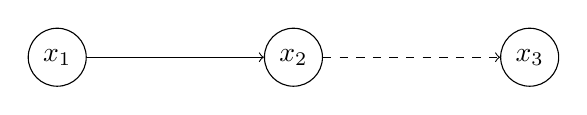
\begin{tikzpicture}
        % Nodes
        \node (x1) [circle, draw] at (0,0) {\(x_1\)};
        \node (x2) [circle, draw] at (3,0) {\(x_2\)};
        \node (x3) [circle, draw] at (6,0) {\(x_3\)};
        
        % Edges
        \draw[->] (x1) -- (x2);
        \draw[dashed, ->] (x2) -- (x3);
    \end{tikzpicture}
\end{center}
\vspace{0.5cm}

whose factorization reads as 

$$
p(x) = \frac{1}{Z}\Psi_{1,2}(x_1,x_2)\dots \Psi_{n-1,n}(x_{n-1},x_n)
$$

Our goal is to maximize $p(x)$ w.r.t. $x_n$.

It is possible to distribute the factorization so that only local computations are required:

$$
\begin{array}{rl}
    \max_{x}p(x) &= \max_{x_1}\dots \max_{x_n}p(x) \\
    &= \frac{1}{Z}\max_{x_1}\max_{x_2}\Psi_{1,2}(x_1,x_2)\dots \max_{x_{n-1}}\Psi_{n-2,n-1}(x_{n-2},x_{n-1})\max_{x_n}\Psi_{n-1,n}(x_{n-1},x_n)
\end{array}
$$

This happens because of the distributive properties of the max, indeed it holds that, given $a > 0$:
\begin{itemize}[label=$\blacktriangleright$, left=0.5cm]
    \item the max distributes over the product 
    
    $$
    \max(ab,ac) = a\cdot \max(b,c)
    $$
    
    \item the max distributes over the sum 
    
    $$
    \max(a+b,a+c) = a + \max(b,c)
    $$
\end{itemize}

This allows us to take an approach similar to the one used in the sum-product algorithm.

Actually we will maximize $\log p(x)$. hence turning the product into sum of logarithms (and this justifies the name max-plus), i.e. our objective is to maximize 

$$
\log p(x) = \sum_i \log \Psi_{i,i+1}(x_i,x_{i+1}) - \log Z
$$

This saves us from product of factors that are possibly very small, since they are probabilities. 

Max-plus algorithm is very similar to sum-product: essentially max replaces sum and plus replaces product. This leads to the following scenarios:

\begin{minipage}{0.45\textwidth}
    \centering
    \includegraphics[width=0.8\textwidth]{assets/fig56.png}   
\end{minipage}
\hfill
\begin{minipage}{0.45\textwidth}
    $$
    \begin{array}{rl}
        \mu_{f\to x}(x) &= \max_{x_1,\dots,x_k}\left[\log f(x,x_1,\dots,x_k) \right. \\
        &\left. + \sum_{x_i\in \mathcal{N}(y)\backslash x}\mu_{x_i\to f}(x_i)\right]
    \end{array}
    $$
\end{minipage}

\begin{minipage}{0.45\textwidth}
    \centering
    \includegraphics[width=0.8\textwidth]{assets/fig57.png}   
\end{minipage}
\hfill
\begin{minipage}{0.45\textwidth}
    $$
    \mu_{x\to f}(x) = \sum_{f_i\in \mathcal{N}(x)\backslash f}\mu_{f_i\to x}(x) 
    $$
\end{minipage}

With base cases:
\begin{itemize}[label=$\blacktriangleright$, left=0.5cm]
    \item $x$ leaf node: $\mu_{x\to f}(x) = 0$
    \item $f$ leaf node: $\mu_{f\to x}(x) = \log f(x)$
\end{itemize}

In order to find the maximum of the joint distribution, that is 

$$
p_{max} = \max_{x_{root}}\left[\sum_{f\in \mathcal{N}(x_{root})}\mu_{f\to x_{root}(x_{root})}\right]
$$

we just need to run the forward pass of the algorithm (i.e. we propagate messages from the leaves up to the root, as in the sum-product algorithm).

\textbf{Remark.} The result will be the same irrespective of which node is chosen as the root.

However, we want to find also the configuration of the variables for which the maximum is achieved. This can be done by applying a slight variation in the forward pass, meaning that we also need to keep track of which values of the variables gave rise to the maximum state of each variable. So during the forward pass we will also store:

$$
\Phi_{f\to x}(x) = \argmax{x_1,\dots,x_k \in \mathcal{N}(f)\backslash x}\left[\log f(x,x_1,\dots,x_k) + \sum_{x_i\in \mathcal{N}(f)\backslash x}\mu_{x_i\to f}(x_i)\right]
$$

Hence, since at the end of the forward pass we know the most probable value of the root node 

$$
x_{root}^{max} = \argmax{x_{root}}\left[\sum_{f\in \mathcal{N}(x_{root})}\mu_{f\to x_{root}}(x_{root})\right]
$$

we can exploit the additional information that we stored to retreive the most probable state of the internal nodes by \textbf{back-tracking}, i.e. by following $\Phi$. For example, assuming the variable nodes connected to $f$ are $x_1,\dots,x_k,x_{root}$, in the first backtracking step we will fix the value of $x_1,\dots,x_k$ according to 

$$
\Phi_{f\to x_{root}}(x_{root}^{max}) = \left\{
    \begin{array}{c}
        x_1 \to x_1^{max} \\
        \dots \\
        x_K \to x_k^{max} \\
    \end{array}
\right\}
$$

and then propagate backwards following $\Phi$ from the other factor nodes connected to $x_1,\dots,x_k$.

\begin{exampleblock}
Consider the following chain:
\vspace{0.5cm}
\begin{center}
    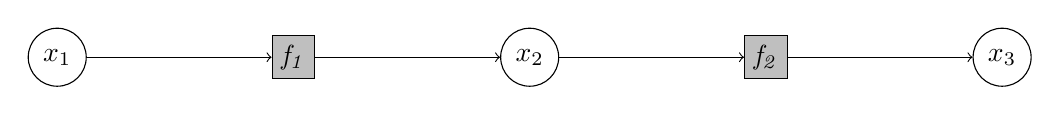
\begin{tikzpicture}
        % Nodes
        \node (x1) [circle, draw] at (0,0) {\(x_1\)};
        \node (f1) [rectangle, draw, fill=gray!50] at (3,0) {\(\mathit{f_1}\)};
        \node (x2) [circle, draw] at (6,0) {\(x_2\)};
        \node (f2) [rectangle, draw, fill=gray!50] at (9,0) {\(\mathit{f_2}\)};
        \node (x3) [circle, draw] at (12,0) {\(x_3\)};
        
        % Edges
        \draw[->] (x1) -- (f1);
        \draw[->] (f1) -- (x2);
        \draw[->] (x2) -- (f2);
        \draw[->] (f2) -- (x3);
    
    \end{tikzpicture}
\end{center}
in which variables are binary, i.e. $x \equiv x_1,x_2,x_3 \in \{0,1\}$ and factors are defined as:

$$
\begin{array}{c}
    f_1(x_1,x_2) = \left[\begin{array}{cc}
        0.3 \\
        0.2 \\
        0.1 \\
        0.4
    \end{array} \right] \text{ where } (x_1,x_2) = \begin{array}{c}
        (0,0) \\
        (0,1) \\
        (1,0) \\
        (1,1)
    \end{array} \\
    f_2(x_2,x_3) = \left[\begin{array}{cc}
        0.1 \\
        0.5 \\
        0.2 \\
        0.2
    \end{array} \right] \text{ where } (x_2,x_3) = \begin{array}{c}
        (0,0) \\
        (0,1) \\
        (1,0) \\
        (1,1)
    \end{array} \\
\end{array}
$$

We start by computing the forward messages edge by edge:

$$
\begin{array}{c}
    \mu_{x_1 \to f_1}(x_1) = 0 \\
    \mu_{f_1 \to x_2}(x_2) = \max_{x_1}[\log f_1(x_1,x_2) + \mu_{x_1 \to f_1}(x_1)] = \left[\begin{array}{c}
        \log 0.3 \\
        \log 0.4
    \end{array}\right] \text{ where } x_2 = \begin{array}{c}
        0 \\
        1
    \end{array} \\
    \mu_{x_2 \to f_2}(x_2) = \mu_{f_1 \to x_2}(x_2) \\
    \mu_{f_2 \to x_3}(x_3) = \max_{x_2}[\log f_2(x_2,x_3) + \mu_{x_2 \to f_2}(x_2)] = \left[\begin{array}{c}
        \log 0.2 + \log 0.4 \\
        \log 0.5 + \log 0.3
    \end{array}\right] \text{ where } x_3 = \begin{array}{c}
        0 \\
        1   
    \end{array} \\
\end{array}
$$

as well as backtracking functions:

$$
\begin{array}{c}
    \Phi_{f_1 \to x_2}(x_2) = \left[\begin{array}{c}
        0 \\
        1
    \end{array}\right] \text{ where } x_2 = \begin{array}{c}
        0 \\
        1
    \end{array} \\
    \Phi_{f_2 \to x_3}(x_3) = \left[\begin{array}{c}
        0 \\
        1
    \end{array}\right] \text{ where } x_3 = \begin{array}{c}
        0 \\
        1
    \end{array} \\
\end{array}
$$

At this point, we can write down the \textbf{lattice/trellis diagram}:

\begin{center}
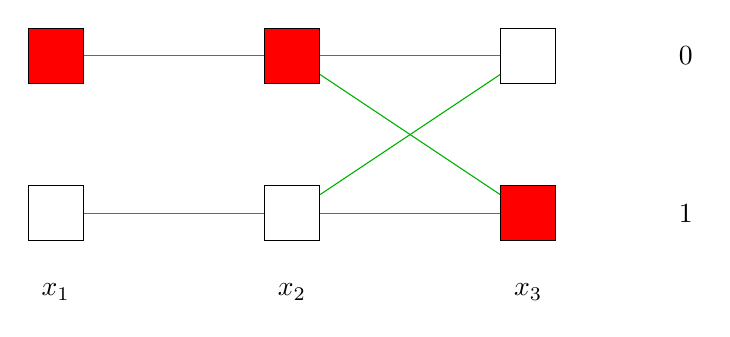
\begin{tikzpicture}[scale=1]
    % Define the nodes (squares)
    % Row 0 (top row)
    \node[draw, minimum size=0.7cm, fill=red] (x10) at (0,0) {};
    \node[draw, minimum size=0.7cm, fill=red] (x20) at (3,0) {};
    \node[draw, minimum size=0.7cm] (x30) at (6,0) {};
    \node at (8,0) {0};
    
    % Row 1 (bottom row)
    \node[draw, minimum size=0.7cm] (x11) at (0,-2) {};
    \node[draw, minimum size=0.7cm] (x21) at (3,-2) {};
    \node[draw, minimum size=0.7cm, fill=red] (x31) at (6,-2) {};
    \node at (8,-2) {1};
    
    % Variable labels
    \node at (0,-3) {$x_1$};
    \node at (3,-3) {$x_2$};
    \node at (6,-3) {$x_3$};
    
    % Draw lines
    % Horizontal lines
    \draw[green!70!black] (x10) -- (x20);
    \draw[green!70!black] (x11) -- (x21);
    
    % Crossed lines
    \draw[green!70!black] (x20) -- (x30);
    \draw[green!70!black] (x21) -- (x31);
    
    % Crossing lines
    \draw[green!70!black] (x20) -- (x31);
    \draw[green!70!black] (x21) -- (x30);
\end{tikzpicture}
\end{center}

This kind of diagram shows explicitly the $K$ (2 in this case) possible states (one per row of the diagram) for each of the variables $x_i$ in the model. The two paths through the lattice correspond to configurations that give the global maximum of the joint probability distribution.

If, for example, we get that:

$$
\begin{array}{c}
    
\max_{x_3}\mu_{f_2\to x_3}(x_3) = \log 0.5 + \log 0.3 \\
\argmax{x_3} = 1
\end{array}
$$

then we can obtain the tuple that maximizes our joint density by following the path backward in the diagram above (we are guaranteed that this path is unique), starting from $x_3 = 1$, i.e. $(0,0,1)$ (red path in the figure). 

\textbf{Note}: in the context of Hidden Markov Models, the max-plus algorithm is called \textit{Viterbi algorithm}.

\end{exampleblock}

\section{Inference in general Probabilistic Graphical Models}

In what follows, we want to extend what we have seen so far to general
probabilistic graphical models, meaning Factor Graphs which contain
loops.

In these cases, we cannot identify the root and the leaves, hence we don’t
have well defined forward and backward directions.

There are several possibilities:
\begin{itemize}[label=$\blacktriangleright$, left=0.5cm]
    \item \textbf{Junction Tree algorithm}: it roughly builds a tree over the cliques
    of the Factor Graph, then exact inference is done in this tree. The
    worst case complexity of this algorithm is exponential in the size
    of the largest clique (so possibly very heavy computationally);
    \item \textbf{Loopy Belief Propagation}: forward and backward pass of the
    sum-product algorithm are iterated several times, until a fix point
    is reached. Unfortunately there is no guarantee that the algorithm
    will converge. When it does, it provides an approximate answer to
    the inference problem;
    \item \textbf{Monte Carlo Sampling}: a general strategy for approximate inference based on sampling;
    \item \textbf{Variational Inference}: it approximates the posterior distribution
    with a simpler distribution belonging to a pre-specified (parametric)
    class, which is the closer one to the true posterior, minimizing the
    KL-divergence.
\end{itemize}



